\begin{task}{5, Bifurcations in crowd dynamics}
In this task we want to apply our knowledge about bifurcation theory to analyze and describe a given SIR model from \cite{shan2014bifurcations}. Unless mentioned all tests were performed with the following values:
\begin{align*}
    A = 20,
    d = 0.1,
    \nu = 1,
    \mu_0 = 10,
    \mu_1 = 10.45,
    \beta = 11.5,
    b = 0.022
\end{align*}

\paragraph{Task 5.1: Setup description}
For this task \verb|sir_model.py| and \verb|sir_bed_model_unfinished.ipynb| were used as code framework. Apart from adding the needed documentation we decided to put the plotting from the python notebook into separate functions. These functions can be found in \verb|sir_model_visualization.py|. This makes the code more readable and modular for later use when creating multiple plots of the SIR simulation.

\paragraph{Task 5.2: Model implementation}
Due to moving the plotting functions into a separate python file, the imports were moved as well. The python notebook only needs to import \verb|sir_model_visualization|.

The differential equation based model from \cite{shan2014bifurcations} was implemented according to the exercise sheet in the \verb|model(...)| function in \verb|sir_model.py|.

\paragraph{Task 5.3: Experiments}
In this task we are observing multiple graphs of the SIR simulation as well as its trajectories. For readability we only use a selected choice of plots, but a more extensive collection can be found in the python notebook \verb|sir_bed_model-t5_3.ipynb|. For this we used different initial values $(S_0, I_0, R_0 )$ for the simulation. Here the $S_0$ is the amount of susceptible, $I_0$ the amount of infected and $R_0$ the amount of removed people at $t=0$. We tested with the following initial values.

\begin{align*}
    (195.3,0.052,4.4), (195.7, 0.03, 3.92), (193, 0.08, 6.21)
\end{align*}

We then observed the graphs for a diverse range of the variable $b$, which is the number of hospital beds per 10,000 persons \cite{shan2014bifurcations}. We performed observations for $b\in\{ 0.01, 0.03\}$ in increments of $0.001$. By doing this we can observe a special kind of bifurcation.

In figure \ref{fig:t5_3-trajB} we present a selected choice of the trajectories plotted in 3 dimensions. Here opaque plot lines in red were added. In figure \ref{fig:t5_3-trajB}(b) for $b=0.022$ we can observe a bifurcation. This is indicated by figure \ref{fig:t5_3-trajB}(a) and \ref{fig:t5_3-trajB}(c), where we observe the trajectories before and after this critical point and see 2 different trajectories for the systems stability. Corresponding to the trajectory for $b=0.022$ we see in figure \ref{fig:t5_3-trajB}(d) further plots.

The first plot in \ref{fig:t5_3-trajB}(d) plots the $S,I,R$ counts over time $t$. We can observe a periodic behaviour for these $S,I,R$ counts over time. For $b=0.020$ we would observe a high amplitude at $t=0$ which decays over time. For $b=0.024$ we observe the opposite case with a small amplitude at $t=0$ which grows larger over time. For border cases with $b=0.01$ or $b=0.03$ we observe the periodic behaviour practically vanishing from the graph.

In the second plot of \ref{fig:t5_3-trajB}(d) we show recovery rate and infected counts plotted over time. Similar to the first plot we observe the same periodic behaviour. It is noteworthy that for $b=0.22$ we have seemingly a stable state where the plotted graphs behave like a periodic functions. Unlike this for $b\neq 0.022$ the graphs instead reach a constant value over time $t$.

The last plot in figure \ref{fig:t5_3-trajB}(d) shows the indicator function $h(I)$. As described in \cite{shan2014bifurcations} section 4.2 essentially $h(I)=0$ is a necessary condition for a Hopf bifurcation. We can observe $h(I)=0$ at two points. This functions is defined as
\begin{align*}
    c_0 &= b^2dA\\
    c_1 &= b((\mu_0 -\mu_1 +2d)A + (\beta -\nu )bd)\\
    c_2 &= (\mu_1 -\mu_0)b\nu + 2bd(\beta-\nu)+dA\\
    c_3 &= d(\beta -\nu )\\
    h(I) &= c_0 + c_1 I + c_2 I^2 + c_3 I^3
\end{align*}

In figure \ref{fig:t5_3-sims}(a) and (b) we see the trajectories of for the initial values $(S_0, I_0, R_0 )=(195.7, 0.03, 3.92)$ and $(S_0, I_0, R_0 )=(193, 0.08, 6.21)$ at $b=0.022$. Their corresponding graphs are also showing the periodic behaviour we have observed in figure \ref{fig:t5_3-trajB}(d). We observe that for different starting values  $(S_0, I_0, R_0 )$ the trajectories take a different form. Similar to the Hopf bifurcation in \ref{fig:t5_3-trajB}(b) we see blue and red dots in figures \ref{fig:t5_3-sims}(a) and (b).

\begin{figure}[H]
\centering
\subfigure[$b=0.020$]{
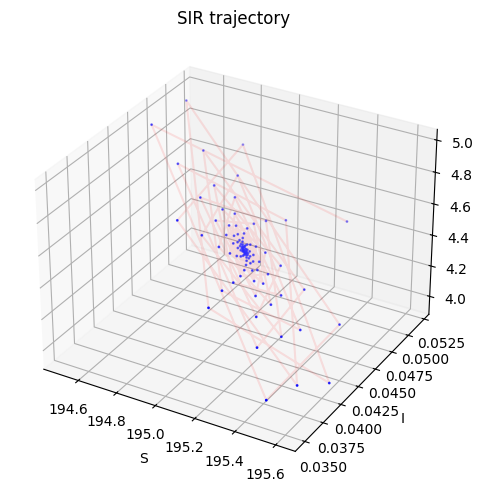
\includegraphics[width=0.3\textwidth]{images/t5_3-traj20.png}}
%\subfigure[$b=0.020$]{
%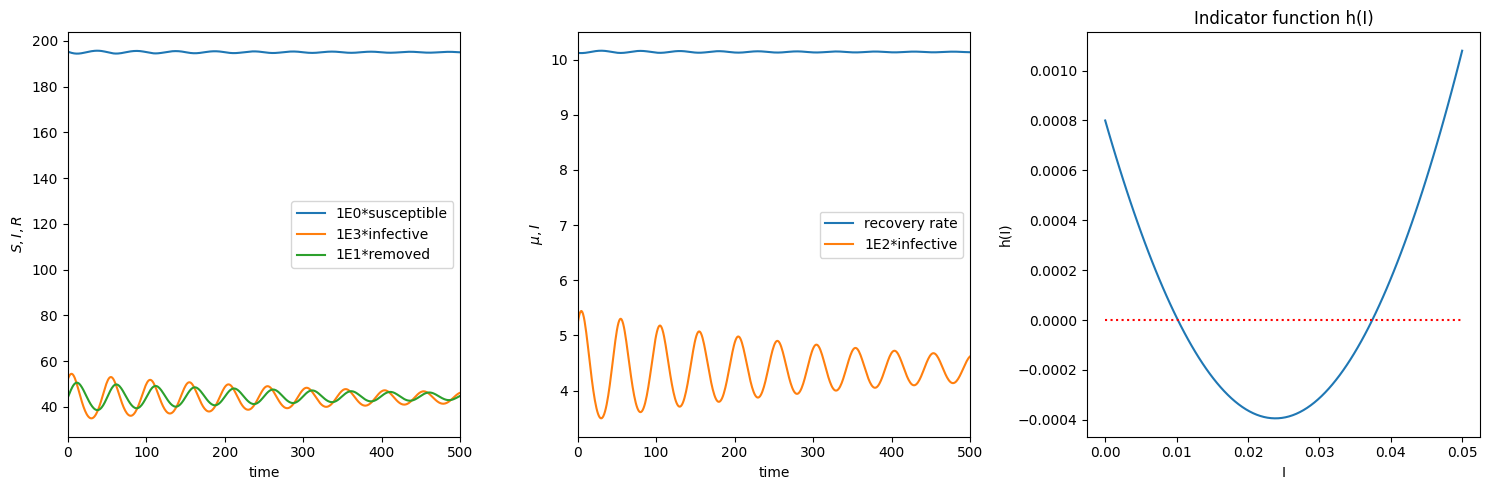
\includegraphics[width=0.6\textwidth]{images/t5_3-sim20.png}}
\subfigure[$b=0.022$]{
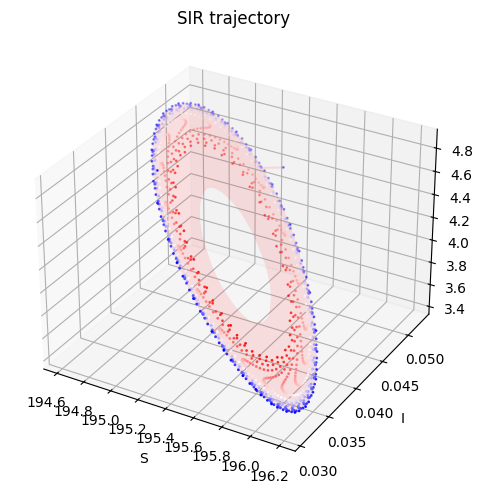
\includegraphics[width=0.3\textwidth]{images/t5_3-traj1.png}}
%\subfigure[$b=0.022$]{
%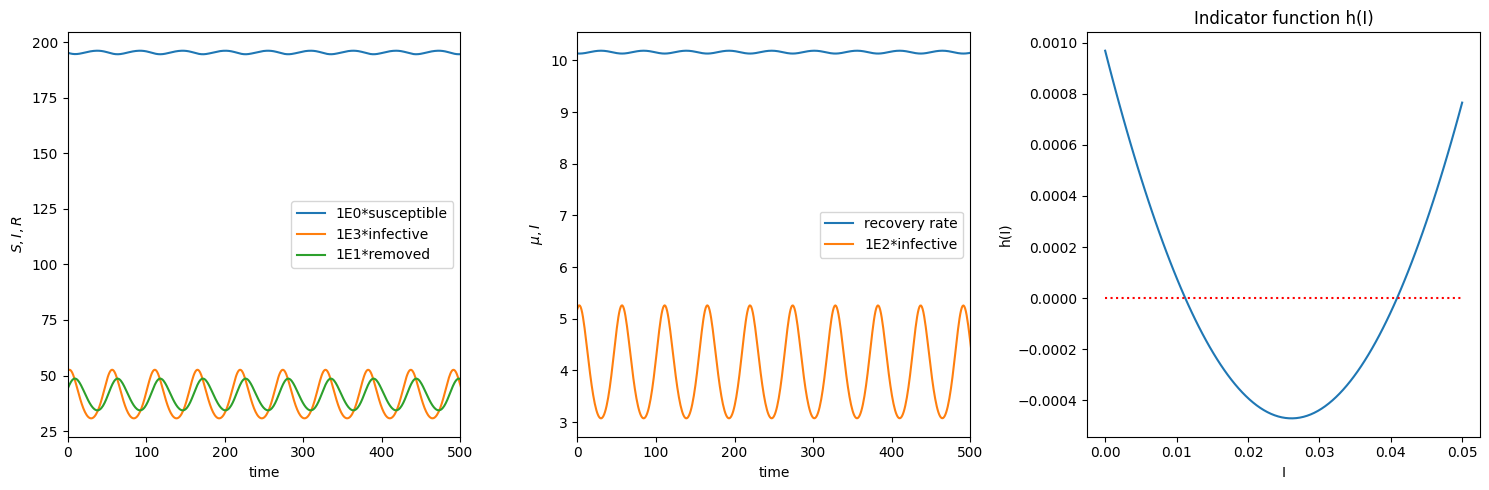
\includegraphics[width=0.6\textwidth]{images/t5_3-sim1.png}}
\subfigure[$b=0.024$]{
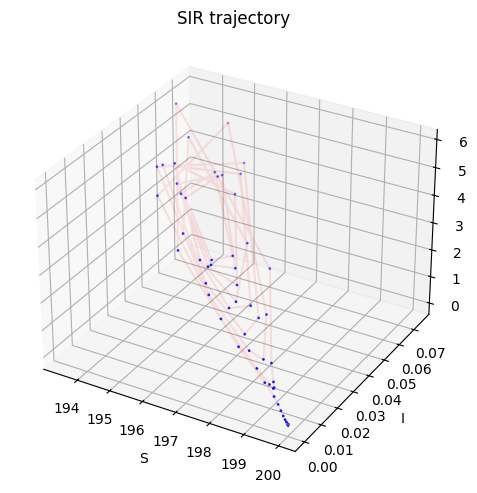
\includegraphics[width=0.3\textwidth]{images/t5_3-traj24.png}}
%\subfigure[$b=0.024$]{
%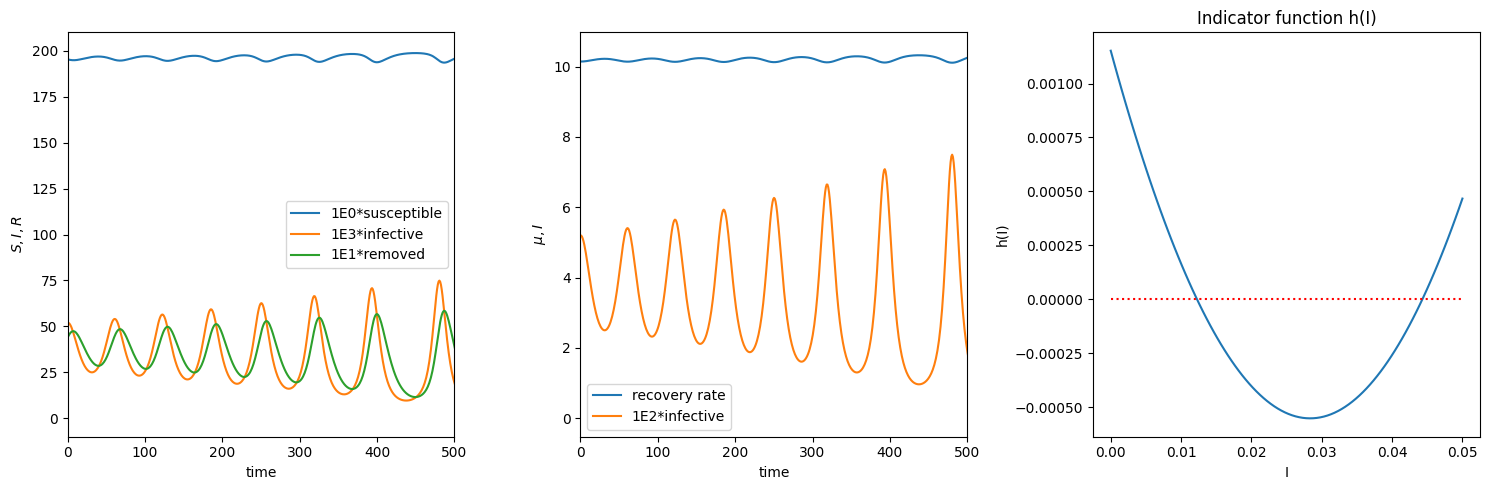
\includegraphics[width=0.6\textwidth]{images/t5_3-sim24.png}}
\subfigure[$b=0.022$]{
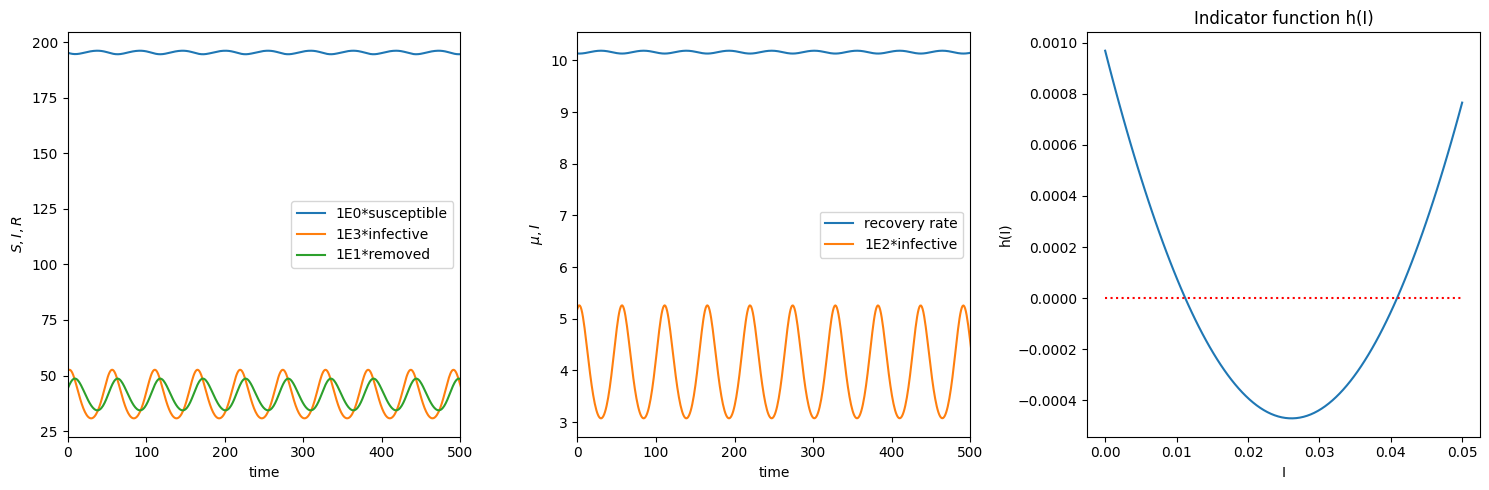
\includegraphics[width=0.9\textwidth]{images/t5_3-sim1.png}}
\caption{Plots for $(S_0, I_0, R_0 )=(195.3,0.052,4.4)$ and different $b$}
\label{fig:t5_3-trajB}
\end{figure}

\begin{figure}[H]
\centering
\subfigure[$(S_0, I_0, R_0 )=(195.7, 0.03, 3.92)$]{
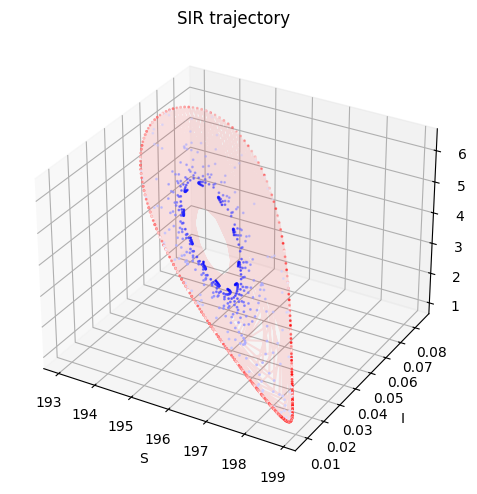
\includegraphics[width=0.3\textwidth]{images/t5_3-traj2.png}}
\subfigure[$(S_0, I_0, R_0 )=(193, 0.08, 6.21)$]{
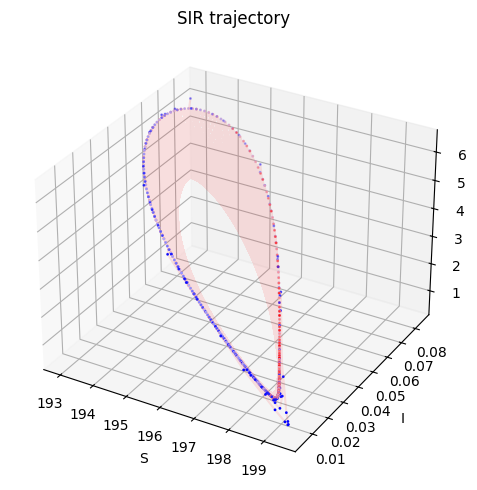
\includegraphics[width=0.3\textwidth]{images/t5_3-traj3.png}}
\caption{Plots for $b=0.022$ and other initial values $(S_0, I_0, R_0 )$}
\label{fig:t5_3-sims}
\end{figure}

\newpage
\paragraph{Task 5.4}
We observe the Hopf bifurcation at $b=0.022$. From the abstract of \cite{rosales2004hopf} "a Hopf bifurcations occurs as a spiral point switches from stable to unstable (or vice versa) and a periodic solution appears". In Figures \ref{fig:t5_3-trajB}(a) to (c) we see a spiral point switch from stable to unstable state. We see the periodic solution in first 2 figures of \ref{fig:t5_3-trajB}(d). But also from \cite{shan2014bifurcations} theorem 4.4 is proven i.e a generic Hopf bifurcation could occur. Then examples are provided as $(195.3, 0.052, 4.4)$ spirals inward to a stable focus (see \ref{fig:t5_3-trajB}(b)), $(195.3, 0.052, 4.4)$ spirals inward to the stable focus (see \ref{fig:t5_3-sims}(a)) and $(193, 0.08, 6.21)$ spirals inward to a stable limit cycle (see \ref{fig:t5_3-sims}(b)).

From \cite{Kuznetsov1998} page 84 the normal-form of the Hopf Bifurcation is defined as:
\begin{align*}
    \begin{cases}
        \dot{x}_1 = \alpha x_1 - x_2 - x_1 (x_1^2 + x_2^2),\\
        \dot{x}_2 = x_1 + \alpha x_2 - x_2 (x_1^2 + x_2^2)
    \end{cases}
\end{align*}

But as evidenced from testing with different parameters we observed that the dynamical system is dependant more than 2 parameters. Looking into \cite{shan2014bifurcations} section 4.3, it is also proven that the cusp type of Bogdanov–Takens bifurcation of codimension 3 occurs at $E_*$. In that section the prove of \cite{shan2014bifurcations} theorem 4.7 leads us to the normal-form:
\begin{align*}
    \begin{cases}
        \dot{X} &= Y,\\
        \dot{Y} &= \epsilon_1 + \epsilon_2 Y+\epsilon_3 XY+X^2 -X^3 Y+\mathcal{O}(|X,Y|^4)Y.
    \end{cases}
\end{align*}

Here $(\epsilon_1, \epsilon_2, \epsilon_3)$ are a function of the bifurcation parameters $(\mu_1, b, \beta)$.

\paragraph{Task 5.5}
From the implementation in \verb|sir_model.py| and \cite{shan2014bifurcations} we can draw the definition of the reproduction number $\mathbb{R}_0$. Here $\beta$ is the average number of adequate contacts per unit time with infectious individuals. $d$ is the per capita natural death rate. $\nu$ is the per capita disease-induced death rate. $\mu_1$ is the maximum recovery rates based on the number of available beds. The reproduction number is defined as the following:
\begin{align*}
    \mathbb{R}_0 = \frac{\beta}{d+\nu +\mu_1}
\end{align*}

Intuitively the reproduction rate $\mathbb{R}_0$ is the ratio between the average contacts with infected individuals per unit time and maximal rate of removing individuals. Essentially the reproduction rate $\mathbb{R}_0$ is the infection rate in relative to the (maximal) removal rate.

From \cite{van2002reproduction} section 3 the reproduction number $\mathbb{R}_0$ is cited as "the expected number of secondary cases produced, in a completely susceptible population, by a typical infective individual". Overall from \cite{van2002reproduction} we can conclude that, if $\beta$ increases or decreases the reproduction rate also increases or decreases. If the reproduction rate is $\mathbb{R}_0<1$, the infection can not grow. If $\mathbb{R}_0>1$ holds, then each infected individual produces more than one new infection on average and hence the infection can spread.

In our previous observations in Figure \ref{fig:t5_3-trajB} all reproduction numbers have been $\mathbb{R}_0 =0.99567 <1$. From \cite{shan2014bifurcations} Theorem 3.3 (4a) the implemented SIR model can have 2 endemic equilibria.

\paragraph{Task 5.6}
The plots for this task can be found in \verb|sir_bed_model-t5_6.ipynb|. We have $(S_0, I_0, R_0) = \mathbb{E}_0 = (A/d, 0,0)$ as initial values and it is obvious that all people become susceptible individuals. First off $S_0 = A/d$ where the count of the susceptible people is $A$ (recruitment/birth rate of susceptible population) divided by $d$ (per capita natural death rate). At the same time, we have no infected $I_0$ or removed $R_0$ individuals. Given this the initial state is disease free. Furthermore, the reproduction rate as defined in the previous section is $\mathbb{R}_0 <1$. Hence we know from \cite{van2002reproduction} section 3 that "on average an infected individual produces less than one new infected individual over the course of its infectious period, and the infection cannot grow".

Therefore the disease-free equilibrium $\mathbb{E}_0 = (A/d, 0,0)$ being an attracting node means that the trajectories in the dynamic system will move to this state. If we look at the figures in \ref{fig:t5_6-plots}(a), we observe all points gathered at the equilibrium $\mathbb{E}_0$ and given the initial values there are no infected and removed people in \ref{fig:t5_6-plots}(b).

Similarly, for $(S,I,R)$ values close to $\mathbb{E}_0$ we assume that all trajectories will lead to this disease-free equilibrium. When performing further testing for $(S,I,R)$ values close to $\mathbb{E}_0$ we can verify that all trajectories lead to the disease-free equilibrium as seen in Figure \ref{fig:t5_6-trajs}(a) to (c). But in Figure \ref{fig:t5_6-trajs}(d) to (f) we can also see that Hopf bifurcation can still occur given specific values. We can verify that $\beta > d+\nu+\mu_0$ holds in our simulations. We thus know from \cite{shan2014bifurcations} theorem 3.3 that $\mathbb{E}_0$ is not globally asymptotically stable, hence bifurcations seen in \ref{fig:t5_6-trajs}(d)-(f) are still possible.

\begin{figure}[H]
\centering
\subfigure[Trajectory of $\mathbb{E}_0$]{
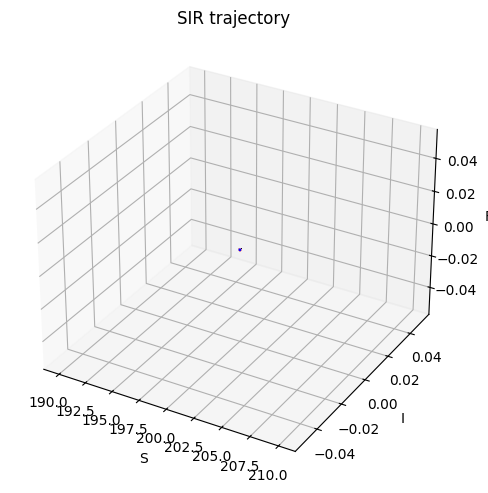
\includegraphics[width=0.3\textwidth]{images/t5_6-traj.png}}
\subfigure[Plots of $\mathbb{E}_0$]{
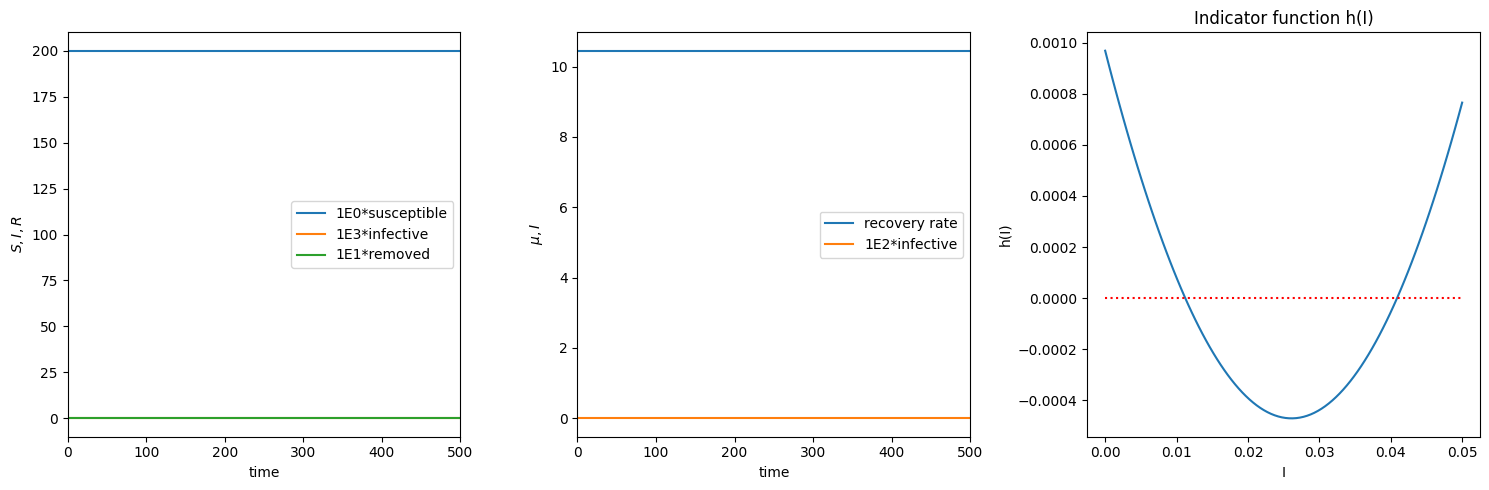
\includegraphics[width=0.6\textwidth]{images/t5_6-sim.png}}
\caption{Plots of disease-free equilibrium $\mathbb{E}_0=(A/d, 0,0)$}
\label{fig:t5_6-plots}
\end{figure}

\begin{figure}[H]
\centering
\subfigure[$(S_0, I_0, R_0) = (200, 0.5, 4.4)$]{
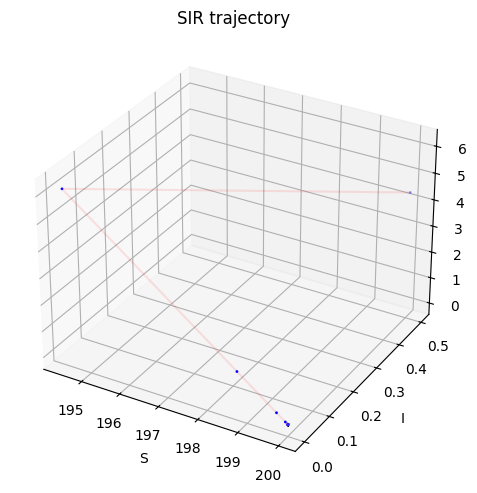
\includegraphics[width=0.3\textwidth]{images/t5_6-traj1.png}}
\subfigure[$(S_0, I_0, R_0) = (200, 0.05, 0.4)$]{
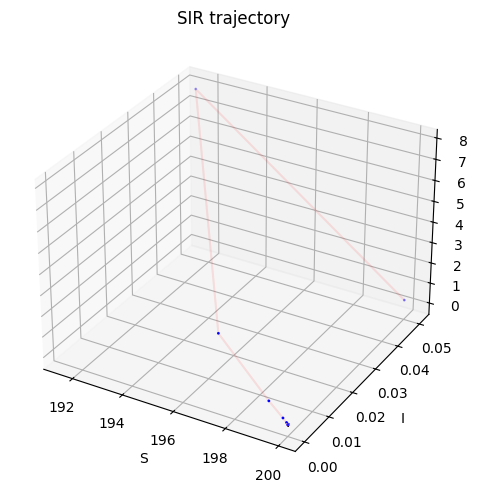
\includegraphics[width=0.3\textwidth]{images/t5_6-traj2.png}}
\subfigure[$(S_0, I_0, R_0) = (200, 0.5, 0.4)$]{
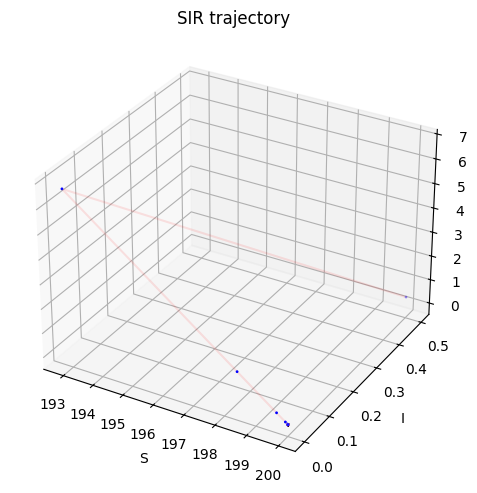
\includegraphics[width=0.3\textwidth]{images/t5_6-traj3.png}}
\subfigure[$(S_0, I_0, R_0) = (200, 0.052, 4.4)$]{
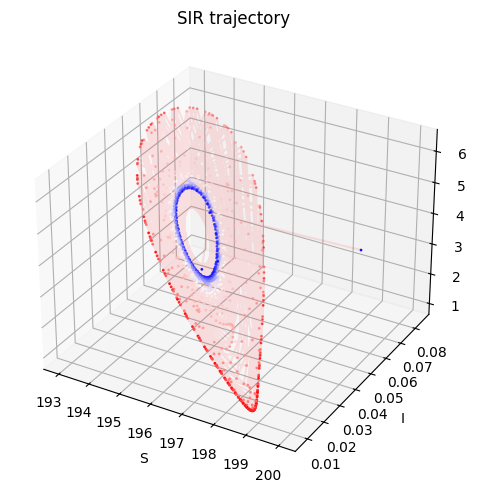
\includegraphics[width=0.3\textwidth]{images/t5_6-traj4.png}}
\subfigure[$(S_0, I_0, R_0) = (200, 0.050, 4.4)$]{
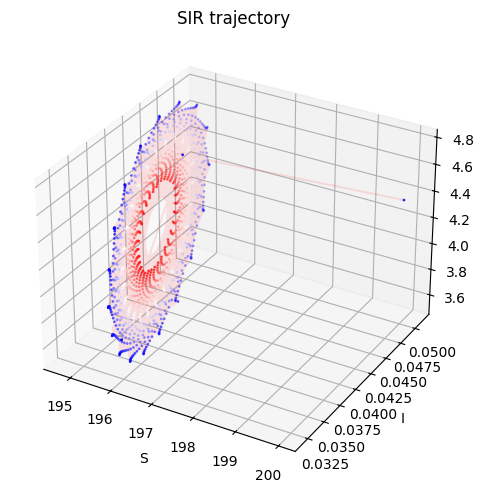
\includegraphics[width=0.3\textwidth]{images/t5_6-traj5.png}}
\subfigure[$(S_0, I_0, R_0) = (200, 0.052, 4.0)$]{
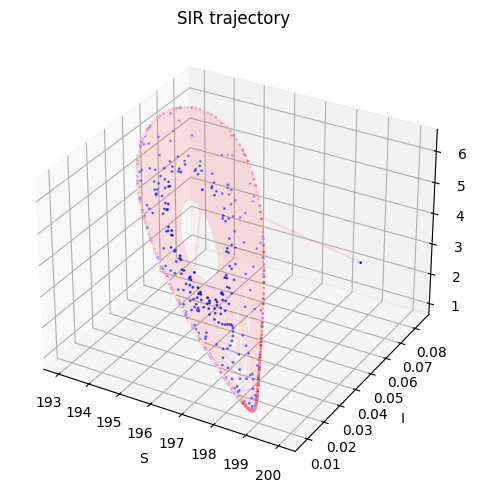
\includegraphics[width=0.3\textwidth]{images/t5_6-traj6.png}}
\caption{Trajectories of $b=0.022$ and $(S_0, I_0, R_0)$ close to $\mathbb{E}_0=(A/d, 0,0)$}
\label{fig:t5_6-trajs}
\end{figure}

\newpage
\paragraph{Task 5.7: Bonus}
For this task the code can be found in the python notebook \verb|sir_bed_model-t5_7.ipynb|. Before we start with the tests we can take note from section 4 Bifurcations in \cite{shan2014bifurcations}. It is shown that the SIR model from \cite{shan2014bifurcations} can undergo the multiple kinds of bifurcations such as:
\begin{itemize}
    \item Forward bifurcation
    \item Backward bifurcation
    \item Pitchfork bifurcation
    \item Saddle-node bifurcation
    \item Hopf bifurcation
    \item Cusp type of Bogdanov–Takens bifurcation
\end{itemize}

 We have previously visualized Hopf bifurcation and in the following we will try to replicate a pitchfork bifurcation. As stated in \cite{shan2014bifurcations} Theorem (4.1) we are considering $\mathbb{R}_0$ as bifurcation parameter. The proof below the theorem  further states that due to the definition of $\mathbb{R}_0$ we can use $\mu_1$ as bifurcation parameter without loss of generality. Then the necessary conditions for a pitchfork bifurcation to occur are namely the following:

\begin{align*}
    \mu_1 &= \beta -d-\nu+\epsilon\\
    b_{pitchfork}:=b &= \frac{A(\mu_1 -\mu_0)}{\beta (\beta -\nu)}\\
\end{align*}

For better comparison we also decided to additionally visualize forward and backward bifurcations. According to theorem 4.1 (1) these are respectively obtained when
$b > \frac{A(\mu_1 -mu_0)}{\beta (\beta -\nu)}$ and $b < \frac{A(\mu_1 -mu_0)}{\beta (\beta -\nu)}$ holds. All parameters are set as given for task 5.3 with exception of the following. In previous iterations of the notebook the initial values $(S_0, I_0, R_0)$ have led to interesting plots, hence these initial values will be used across all experiments. Since $b$ can be chosen arbitrarily we have decided to use similar values as in the paper \cite{shan2014bifurcations} Figure 7 (a) and (b), so that we can potentially obtain similar plots as in the paper. These use $b=0.07$ for forward bifurcation and $b=0.04$ for backward bifurcation.\\

In figures \ref{fig:t5_7-traj}(d)(e)(f) we see their trajectories of each bifurcation when plotting in 3d. Since $R$ axis is not relevant it is easier to analyse the trajectories in the $(S,I)$ plane. This can be seen in \ref{fig:t5_7-traj}(a)(b)(c). Note that the color gradient describes the change of the $(S,I,R)$ values over time $t$. Here $t=0$ is blue and turns white and then into red when reaching the end $t=t_{max}$.

Figure \ref{fig:t5_7-traj}(a) and (d) are the trajectories of the pitchfork bifurcation and unfortunately it is very hard to interpret it. But if we look at the trajectories of the forward (Fig. \ref{fig:t5_7-traj}(b)(e)) and backward bifurcation (Fig. \ref{fig:t5_7-traj}(c)(f)) we can see their similarities as well as their polar behaviour. The opposite development of their trajectories can be simply explained from their relation to the variable $b$. For \ref{fig:t5_7-traj}(b) we could form a correlation that the amount of hospital beds $b>b_{pitchfork}$ leads to a decrease of infected over time (indicated by the coloring) given that the reproduction number is fixed as $\mathbb{R}_0=1$. Similarly observed in \ref{fig:t5_7-traj}(c) $b>b_{pitchfork}$ In infected show an increase behaviour over time. When observing \ref{fig:t5_7-traj}(b)(c) from the perspective of $S$, we observe periodic behaviour. This probably captures the constant, but fluctuating behaviour of the birthrate for $S$. Additionally we can speculate the the existence of this periodic behaviour is what causes Hopf bifurcations.

Combining previous observations we can assume that the pitchfork bifurcation in \ref{fig:t5_7-traj}(a) is the point between forward and backward bifurcation, when it comes to their trajectories. This is further more expanded when observing their trajectories in 3d \ref{fig:t5_7-traj}(d)-(f). We can confirm this behaviour when checking \cite{shan2014bifurcations} Figure 2, where the point $K$ lies between the sets of values $C^+_0$ and $C^-_0$, which represent the $(\mu_1,b)$ tuples when forward and backward bifurcations occur.

\begin{figure}[H]
\centering
\subfigure[Trajectory of Pitchfork Bifurcation]{
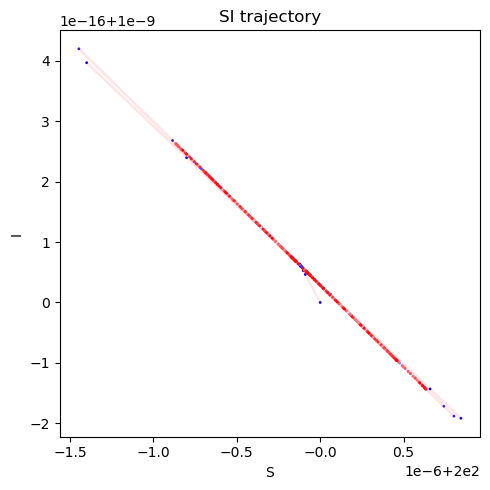
\includegraphics[width=0.3\textwidth]{images/t5_7-pf-traj.png}}
\subfigure[Trajectory of Forward Bifurcation]{
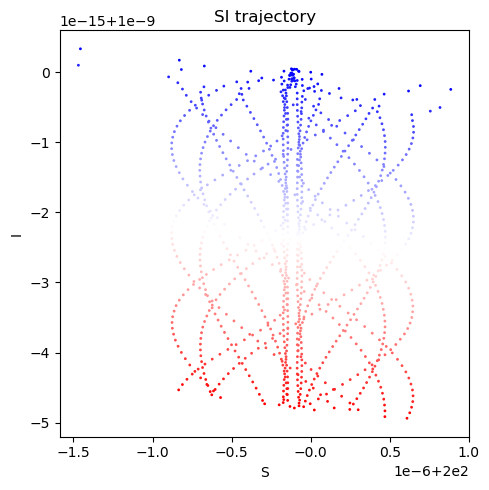
\includegraphics[width=0.3\textwidth]{images/t5_7-fw-traj.png}}
\subfigure[Trajectory of Backward Bifurcation]{
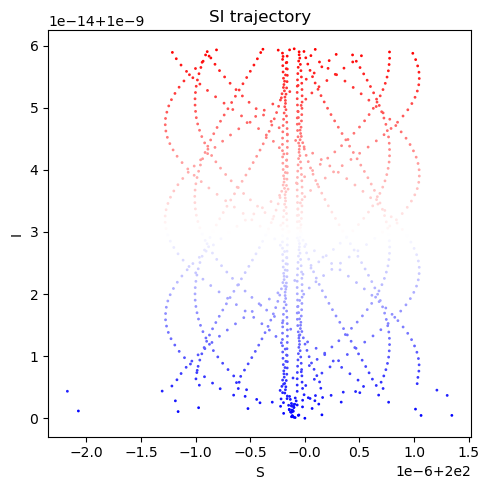
\includegraphics[width=0.3\textwidth]{images/t5_7-bw-traj.png}}
\subfigure[Trajectory of Pitchfork Bifurcation]{
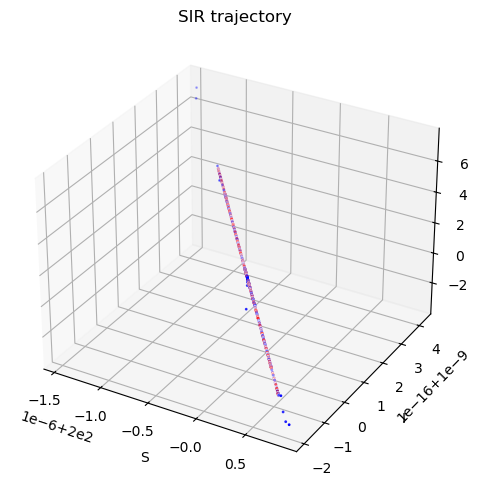
\includegraphics[width=0.3\textwidth]{images/t5_7-pf-traj3d.png}}
\subfigure[Trajectory of Forward Bifurcation]{
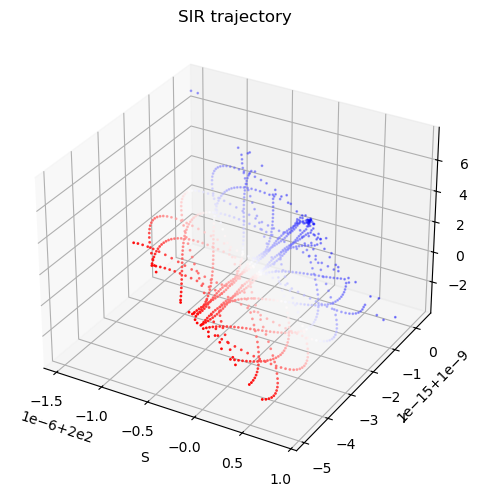
\includegraphics[width=0.3\textwidth]{images/t5_7-fw-traj3d.png}}
\subfigure[Trajectory of Backward Bifurcation]{
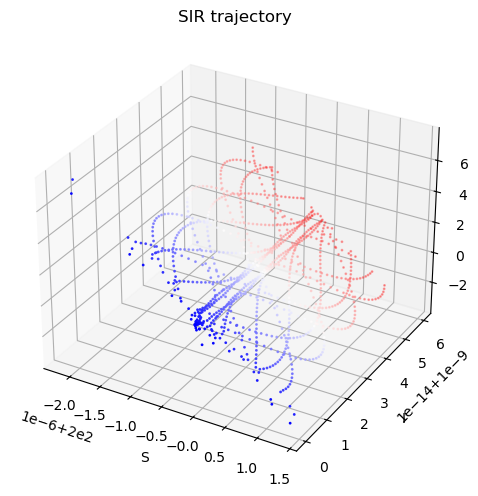
\includegraphics[width=0.3\textwidth]{images/t5_7-bw-traj3d.png}}
\caption{Trajectories in $S,I$ and $S,I,R$ plane}
\label{fig:t5_7-traj}
\end{figure}

Since the trajectories can not paint the full picture, we will next look at their bifurcation diagrams. This idea is inspired by \cite{shan2014bifurcations} Figure 7, since reproducing similar diagrams would confirm that we have plotted the pitchfork bifurcation correctly. In figures \ref{fig:t5_7-R0}(a)(b)(c) the reproduction number $\mathbb{R}_0$ is plotted against $I$. Note that $\mathbb{R}_0$ is treated as bifurcation parameter, but the implementation only change $\mu_1$, affecting $\mathbb{R}_0$ in consequence. Since $\mu_1$ is the bifurcation parameter we need to recalculate the number of infected $I$ every time.

For better understanding of plotting $\mathbb{R}_0$ against $I$ we also plotted it in 3d against $t$ in figures \ref{fig:t5_7-R0}(d)(e)(f). When excluding small $t$-values we can confirm that bifurcation diagram is consistent across all time slices.\\

The initial observation is that all bifurcation diagrams look similar. We can easily confirm that \ref{fig:t5_7-R0}(b) is behaving as expected, when comparing it to \cite{shan2014bifurcations} Figure 7(a). In a forward bifurcation, as the bifurcation parameter crosses a critical threshold, the system transitions from one stable state to another. Before the threshold we are in the disease-free equilibrium and afterwards the onset of the epidemic is seen as $\mathbb{R}_0$ crosses the threshold of 1.

As for backward bifurcation Figure 7(b) from \cite{shan2014bifurcations} shows that the existence of an epidemic extends also for some values below $\mathbb{R}_0<1$. While \ref{fig:t5_7-R0} does not fully capture this (due to implementations haven taken too long up to this point), we can see that the cut-off at $\mathbb{R}=1$ implies this behaviour of the backwards bifurcation.

When looking at \ref{fig:t5_7-R0}(a) we can not that the bifurcation diagram is likely the same as the forward bifurcation. We can say at this point that like the forward bifurcation, the pitchfork bifurcation marks the start of an epidemic as well, when crossing $\mathbb{R}_0$. Unfortunately the pitchfork bifurcation does not show the characteristic pitchfork shape. Logically speaking it wouldn't make sense to observe a decrease in infected individuals given that there is none, while increasing the reproduction number crossing the threshold $\mathbb{R}_0 = 1$. Looking back into \cite{shan2014bifurcations} the proof of theorem 4.1 shows that the set of points describing pitchfork bifurcations can be described using the following:

\begin{align*}
    C^\pm_{\Delta}: b&=f^\pm_{\Delta}(\mu_1)\triangleq\frac{\beta (\mu_1-\mu_0)+\delta_0(\delta_1-\beta)\pm \sqrt{\beta\delta_1(\mu_1-\mu_0)(\delta_1-\beta)}}{(\beta-\nu)\delta_1^2}\\
    \delta_0 &= d+\nu+\mu_0\\
    \delta_1 &= d+\nu+\mu_1
\end{align*}

It can then be verified that then $f^\pm_{\Delta}(\delta-d-\nu)=\frac{A(\mu1-\mu0)}{\beta()\beta-\nu}$ holds. This is verified in the python notebook as well using the functions \verb|f_plus(...)| and \verb|f_minus(...)|. This explains why the pitchfork bifurcation in $\mathbb{R}_0,I$ plane shows the same behaviour as the forward bifurcation. The observe characteristic we would probably instead need to plot $b$ against $\mu_1$ using the definition $b=f^\pm_{\Delta}(\mu_1)$. The curves of $C_0^+$ and $C^-_0$ could be interpreted as the pitchfork.\\

Overall we can see that SIR model described using the differential equations in \cite{shan2014bifurcations}(2.2) is a very complex dynamical system. In this task have observed that different bifurcations can occur given the right settings. As for the pitchfork bifurcation it exists under special conditions such that the forking part overlaps with each other.

\begin{figure}[H]
\centering
\subfigure[Pitchfork Bifurcation at $t=999$]{
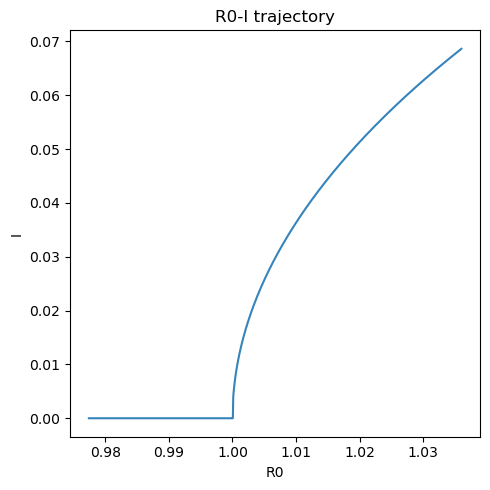
\includegraphics[width=0.3\textwidth]{images/t5_7-pf-R0.png}}
\subfigure[Forward Bifurcation at $t=999$]{
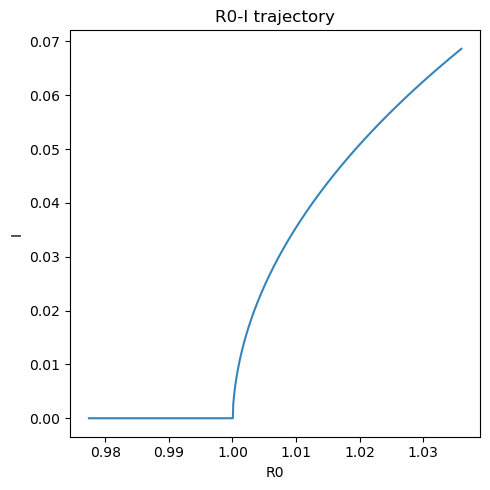
\includegraphics[width=0.3\textwidth]{images/t5_7-fw-R0.png}}
\subfigure[Backward Bifurcation at $t=999$]{
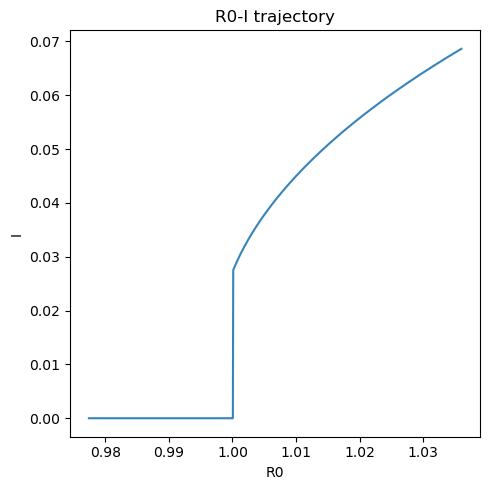
\includegraphics[width=0.3\textwidth]{images/t5_7-bw-R0.png}}
\subfigure[3D plot of Pitchfork Bifurcation]{
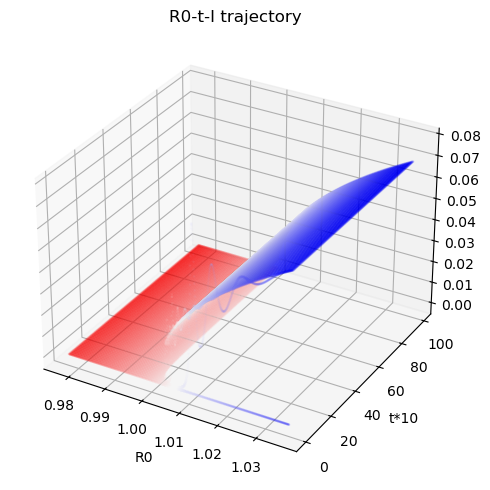
\includegraphics[width=0.3\textwidth]{images/t5_7-pf-R03d.png}}
\subfigure[3D plot of Forward Bifurcation]{
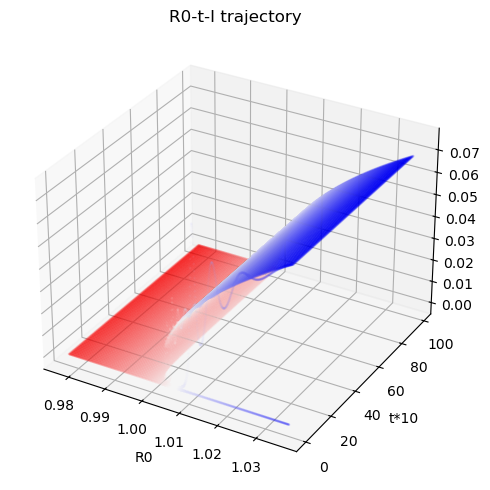
\includegraphics[width=0.3\textwidth]{images/t5_7-fw-R03d.png}}
\subfigure[3D plot of Backward Bifurcation]{
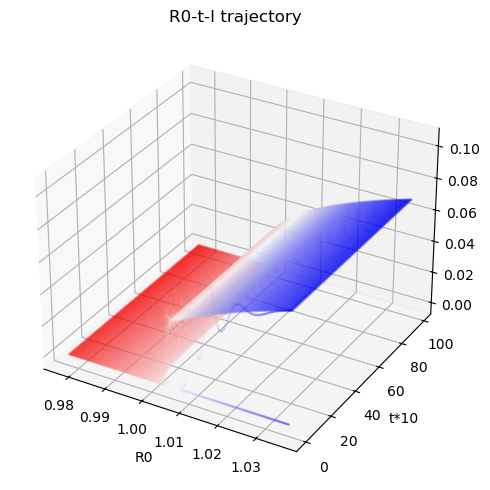
\includegraphics[width=0.3\textwidth]{images/t5_7-bw-R03d.png}}
\caption{Bifurcation diagram on $\mathbb{R}_0, I$ plane}
\label{fig:t5_7-R0}
\end{figure}

\end{task}